\section{KaioKen}

	\subsection{Introducción}
		Sea $n \in \mathds{N}$, $c: conj(lista(nat))$. El objetivo de este problema es encontrar la menor cantidad de listas necesarias que cumplan con las siguientes condiciones: 
		    \begin{itemize}
                \item ($ \forall l \in c$) tam($l$) = $n$
                \item ($ \forall l \in c$) ($ \forall i < n$) $l[i]$ = 1 $\vee$ $l[i]$ = 2
                \item ($ \forall i < n$) ($ \forall j < n$) $\exists$ ($l \in c$) $l[i] \neq l[j]$
            \end{itemize}
    Es decir, todas las listas deben tener tamaño igual a $n$, y sus elementos deben ser 1 o 2. Se trata de minimizar el cardinal del conjunto $c$ cumpliendo con las tres condiciones. 
    Por ejemplo:\\
    
      Para n = 4  \\
    \\

\begin{wrapfigure}{l}{3cm}
  \vspace{-41pt}
  \begin{center}
    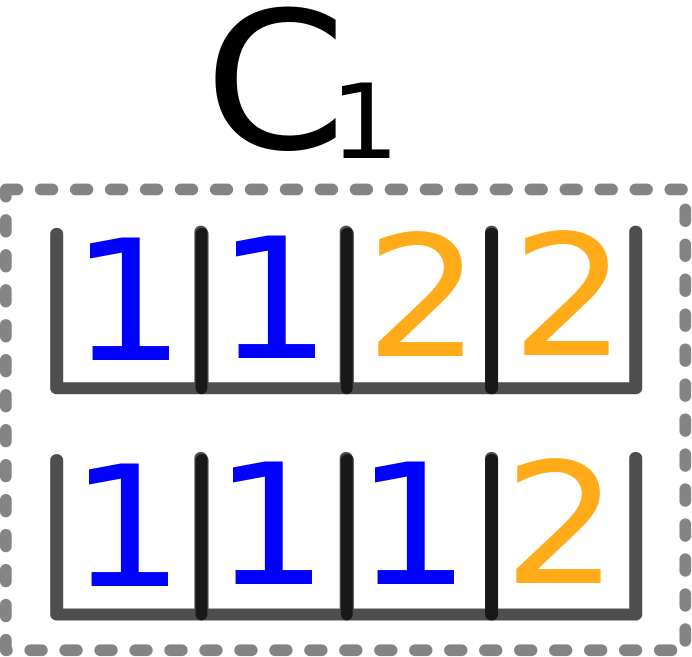
\includegraphics[width=2cm]{graficos/c1.png}
  \end{center}
\end{wrapfigure}

 El conjunto $C_{1}$ no es una solución válida ya que no cumple con la tercera condición. Para $i$=0, $j$=1, no existe una lista $l$ donde $l[i] \neq l[j]$.
\\
\\
\\

\begin{wrapfigure}{l}{3cm}
  \vspace{-41pt}
  \begin{center}
    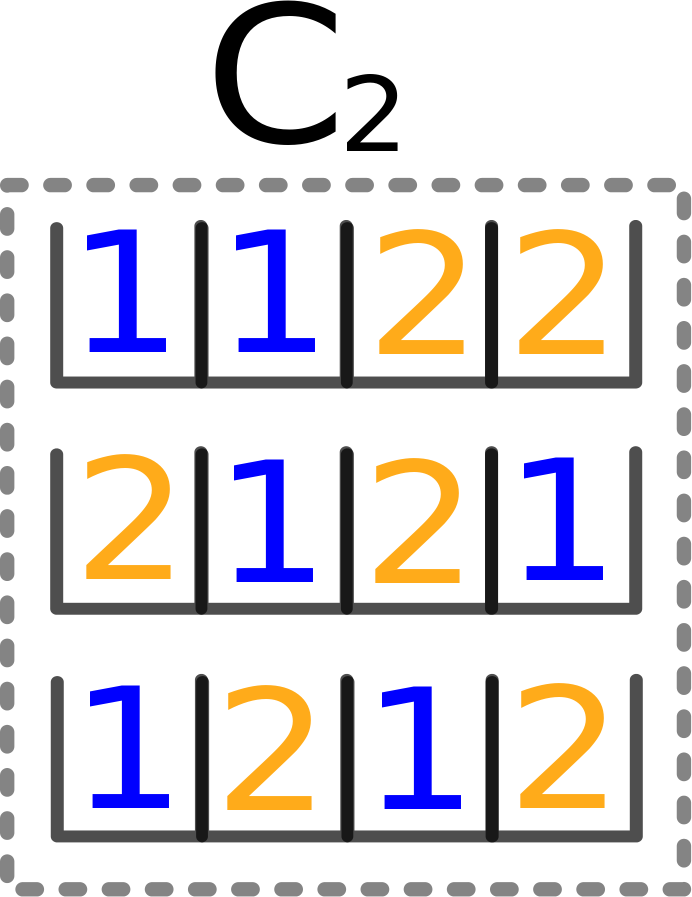
\includegraphics[width=2cm]{graficos/c2.png}
  \end{center}
\end{wrapfigure}

 El conjunto $C_{2}$ tampoco es una respuesta correcta ya que omitiendo alguna de las listas el conjunto sigue cumpliendo con las tres condiciones nombradas anteriormente. \\
 \\
 \\

{\begin{tabular}{ccc}
   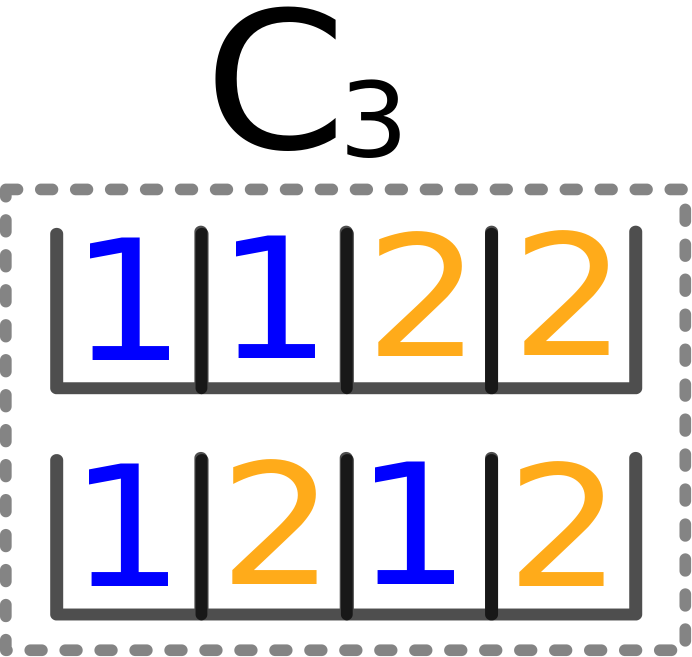
\includegraphics[height=2cm]{graficos/c3.png} & 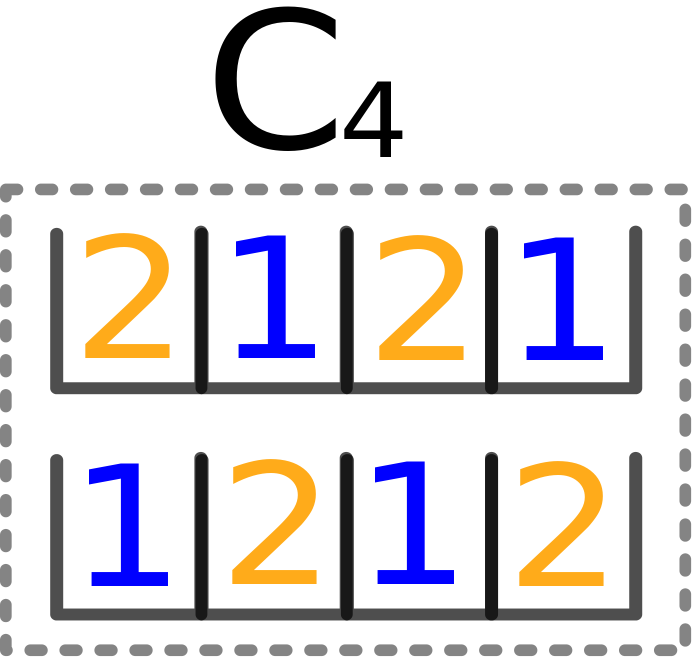
\includegraphics[height=2cm]{graficos/c4.png} & 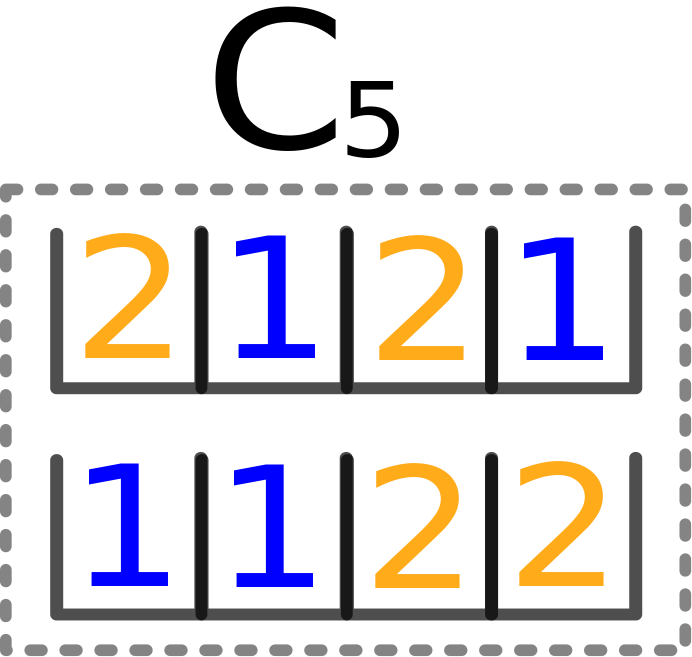
\includegraphics[height=2cm]{graficos/c5.png} \\
   \\

\end{tabular}}

  Los conjuntos $C_{3}$, $C_{4}$ y $C_{5}$ son respuestas válidas. 




    \subsection{Desarrollo}
	La idea del algoritmo es dividir a los peleadores de manera tal que la cantidad de peleas sea $\lceil log_{2}(n) \rceil$ y luego probaremos que esa es la cantidad optima de peleas.\\
   Para esto lo que hara el algoritmo sera hacer pelear inductivamente( sobre la variable i) vectores de a lo sumo $2^{i}$ peleadores y hacerlos pelear todos contra todos(observamos que como el caso de que no sea una potencia de 2 la entrada no afecta a la cantidad de peleas, como probaremos despues,pues $\lceil log_{2}(n) \rceil=log_{2}(2^k)$ con k la potencia de 2 mas chica mayor a n , ni tampoco afecta de nigun modo a la complejidad, porque siempre existe dicho k y es  a lo sumo el doble del numero menos uno, podemos entonces  explicar el algoritmo basado en entradas de a lo sumo$2^{i}$elementos).\\
  La idea del codigo seria entonces la siguiente:\\
  \\
Caso base:\\
   -para i=1, hay una unica pelea pues si tenemos$2^{i}=2$ elementos separo al vector a la mitad y pelean todos contra todos (V[0] vs V[1]).
   observamos que entonces pelearon todos contra todos en $log_2(2^{i}i)=i$ peleas.\\
   \\
Paso recursivo:\\
  -Tomamos el vector vector de $2^{i}$ peleadores, y lo partimos en 2 llamando recursivamente con 2 vectores de $2^{i-1}$ ambos los puedo hacer pelear todos contra todos en tan solo $log_2(2^{i-1})=i-1$ y  de forma que les es indistinta la presencia de los otros $2^{i-1}$ peleadores, asi que en $i-1$ peleas pelearon todos contra todos en los 2 subvectores en sus respectivas llamadas recursivas. faltaria solo agregar una pelea entre que pelean todos los de una mitad contra la otra y tengo entonces una lista de peleas de todos contra todos.
\\
\\
Se observa entonces que pelearon todos contra todos en $log_2(2^{i-1})=i$ peleas que por la aclaracion antes enunciada se trasladaria a que un vector de N peladores pelearia en $\lceil log_{2}(n) \rceil$, resta solo ver para confirmar la correctitud del algoritmo que $\lceil log_{2}(n) \rceil$, es la minima cantidad de pelas requeridas.
\\
Para terminar entonces, vamos a probar que para todo $n$, la menor cantidad de peleas necesarias es $\lceil log_{2}(n) \rceil$ por inducción en $N$.

        Caso Base: N = 1
        Un solo guerrero necesita $0$ peleas para haber peleado con todos los demás, $\lceil log_{2}(1) \rceil$ = $0$.

        Paso Inductivo: Supongo que $\forall$ $K$ $<$ $N$. La menor cantidad de peleas necesarias es $\lceil log_{2}(k) \rceil$. Quiero ver que se cumple también para $N$.

        Caso $N$ par:
        Genero una pelea $P$ de una mitad contra la otra. 

        {\begin{tabular}{ccc}
         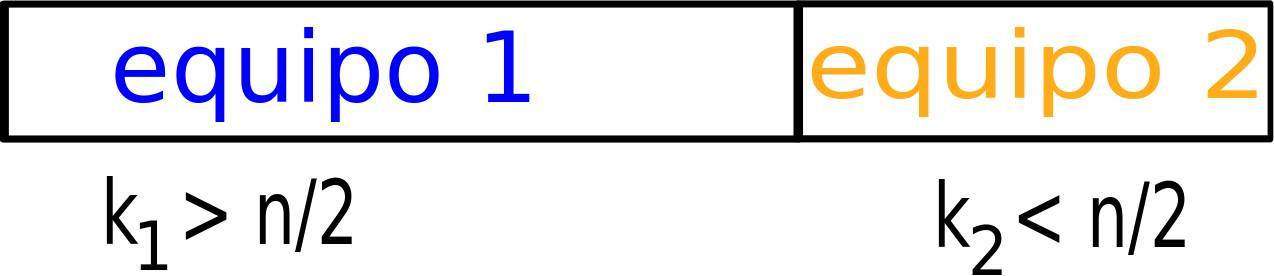
\includegraphics[height=2cm]{graficos/kaioken-desarrollo-1.jpg} 

          \end{tabular}}

        Por Hipótesis Inductiva, cada subgrupo necesitaría $\lceil log_{2}(N/2) \rceil$ peleas para pelearse todos entre sí. Como estas subpeleas pueden hacerse “simultáneamente”, el total de peleas es $\lceil log_{2}(N/2) \rceil$ $+$ $1$. Esto es igual a $\lceil log_{2}(N) \rceil$. \\

        ¿Qué pasa si no divido a la mitad?\\


        GRAFICO 2!!!\\
        \\

        En este caso, la cantidad de subpeleas previas depende de $k_{1}$, el de cantidad mayor entre las dos partes(que es de tamaño por lo menos la mitad). Las peleas anteriores terminan siendo $\lceil log_{2}(k_{1}) \rceil$. Por hipótesis inductiva. Esto es mayor o igual a $\lceil log_{2}(N/2) \rceil$ concluyendo asi la optimalidad de la resolucion. \\

        Caso N Impar: \\
        \\

        GRAFICO 3!!!!
        \\

        Por hipótesis inductiva, podemos hacer pelear cada equipo entre sí en como mínimo $\lceil log_{2}((N-1)/2+1) \rceil$ $=$ $\lceil log_{2}((N+1)/2) \rceil$. Como $N$ es impar, $\lceil log_{2}((N+1)/2) \rceil$ es igual a $\lceil log_{2}(N/2) \rceil$. De esa manera, nos vuelve a quedar como cantidad de peleas total $\lceil log_{2}(N) \rceil$. \\

        Un corte de tamaños distinto a éste genera el mismo resultado que el caso par explicado anteriormente, de donde podemos deducir entonces la optimalidad de la solucion. \;






    \subsection{Complejidad}

    \begin{algoritmo}{kaioken}{int n}{int}

  \tipo{int} $cantMinPeleas \gets \lceil log_{2}(n) \rceil$ \com*{O(1)}
  \tipo{int} $equipo$ \com*{O(1)}

  \For(\com*{O($log_{2}(n)$)}){($i$ = 1; $i \leq cantMinPeleas$; $i$++)}{
    $equipo \gets 1$ \com*{O(1)}
    \For(\com*{O($n/2^{i-1}$)}){($h$ = 1; $h \leq n$; $h$ = $h + 2^{i-1}$)}{
      \For(\com*{O($2^{i-1}$)}){($k$ = 0; ($k < 2^{i-1}$) $\&$ ($h+k \leq n$); $k$++)}{
        escribir($equipo$) \com*{O(1)}
      }
        \eIf(\com*[f]{O(1)}){$equipo == 1$}{
          $equipo \gets 2$ \;
        }{
          $equipo \gets 1$ \;
        }
    }
  }


\end{algoritmo}

El segundo ciclo junto con el tercer ciclo tienen complejidad O($n$), ya que se multiplica O($n/2^{i-1}$) por O($2^{i-1}$). Entre los dos ciclos se recorren todos los guerreros una vez. El segundo recorre por grupos de guerreros que van a pertenecer al mismo equipo y el segundo de ellos le asigna a cada guerrero de un grupo el número de equipo correspondiente. 

Por ejemplo, para $n$=8, el ciclo número dos recorre como indican las flechas rojas para la pelea 1, 2 y 3 respectivamente. El tercer ciclo, avanza por los enemigos entre las flechas rojas. Se puede observar que el vector se recorre una sola vez para cada pelea. 


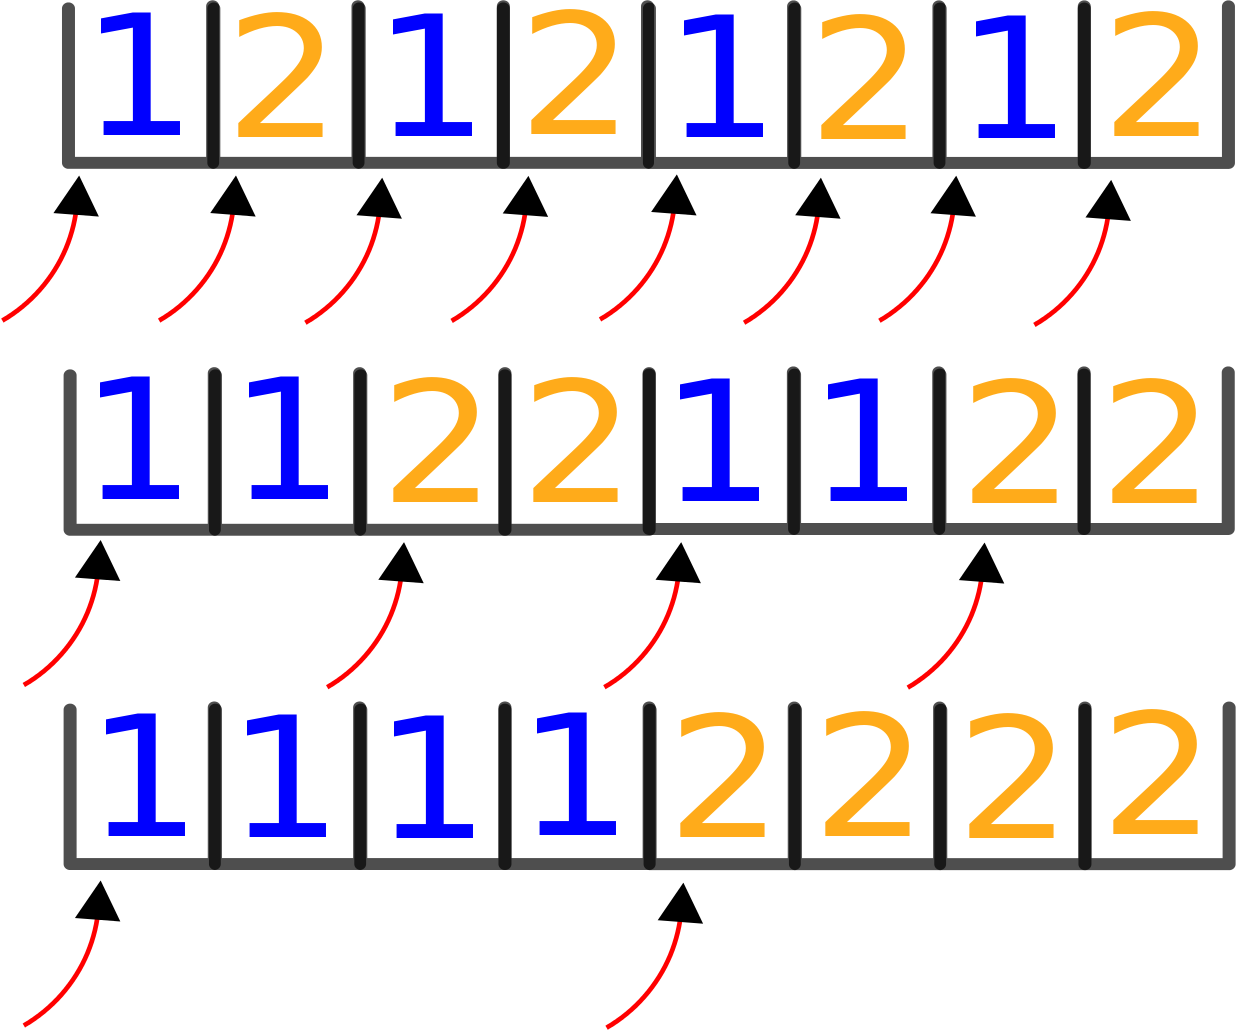
\includegraphics[height=4cm]{graficos/ciclo.png}




    \subsection{Experimentación}
		El objetivo de este experimento fue extraer conclusiones acerca de la variación en el tiempo de cómputo requerido por el algoritmo para distintos valores de $n$, con el fin de determinar su complejidad. 
    Para lograrlo, se graficó la curva $n \times log_{2}n / 13000000$ y se la comparó con las mediciones obtenidas al ejecutar el programa.

    \subsubsection*{Datos de entrada}
    La cantidad guerreros tomados fueron  desde 10000 hasta 300000 de 10000 en 10000.
    El archivo necesario para ejecutar el experimento se encuentra en la carpeta exp/kaioken con nombre kaioken.sh. 
		Para realizar las mediciones se  utilizaron las funciones provistas a tal efecto por la cátedra. Además, para evitar posibles errores en las mismas, cada una se repitió 7 veces, considerando luego el promedio entre los valores obtenidos. 



      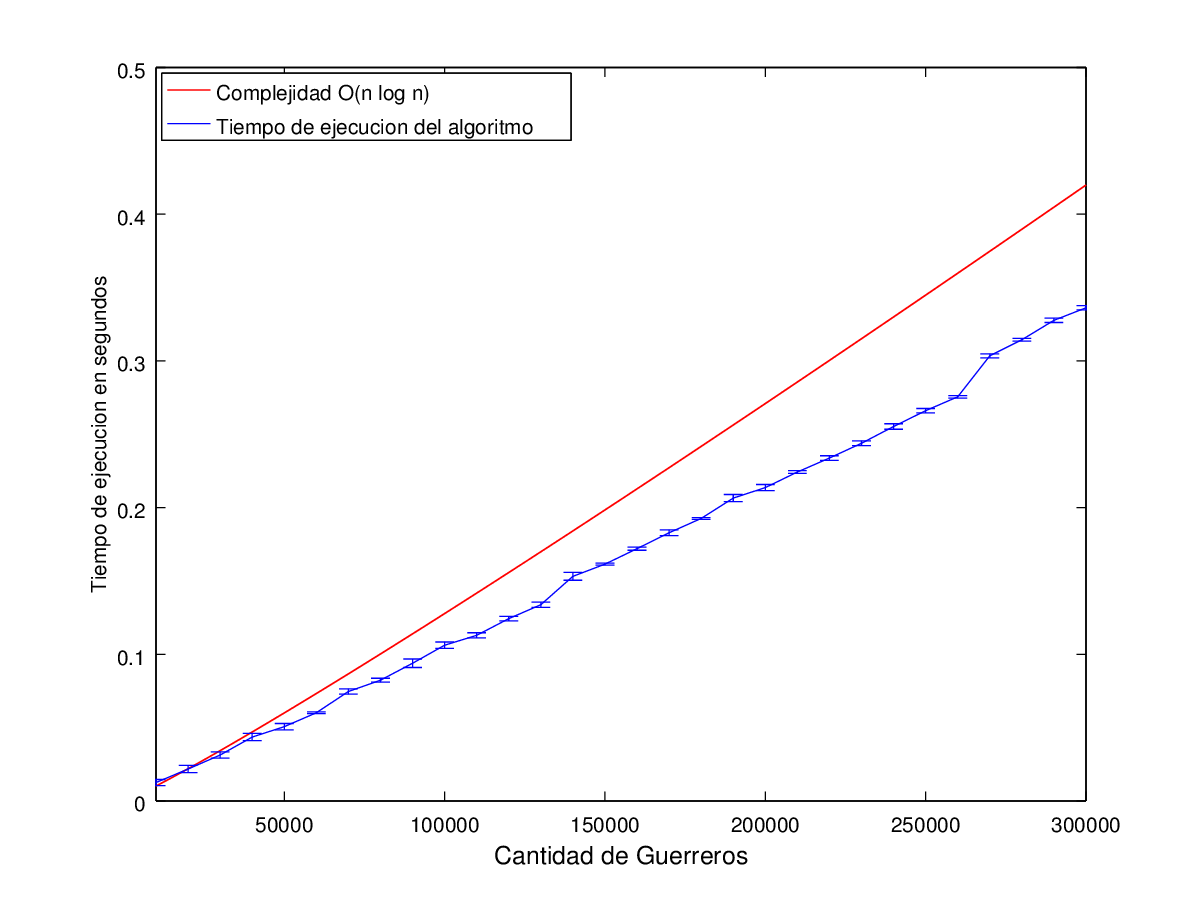
\includegraphics[height=11cm]{graficos/kaioken-exp.png}



		\subsubsection*{Conclusión}
			Se puede observar en el gráfico que la curva $n \times log_{2}n / 13000000$ está por encima de la curva que forman las mediciones del tiempo de ejecución del programa. Por lo tanto, se demuestra empiricamente que la complejidad del programa es O($n \times log_{2}n$)
